\documentclass[a4paper]{scrartcl}

\usepackage{lmodern}
\usepackage[T1]{fontenc}

\usepackage{alltt}
\usepackage{xcolor}
\usepackage{graphicx}
\usepackage{framed}
\usepackage[utf8]{inputenc}
\usepackage{mdwlist}

\DefineNamedColor{named}{Link}{rgb}{0,0,0.3}
\DefineNamedColor{named}{Cite}{rgb}{0,0.3,0}
\DefineNamedColor{named}{URL}{rgb}{0.3,0,0}

% Platz für Gleitobjekte:
\renewcommand\floatpagefraction{.7}
\renewcommand\topfraction{.8}
\renewcommand\bottomfraction{.5}
\renewcommand\textfraction{.2}



\usepackage[
,colorlinks
,linkcolor=Link
,pagecolor=Link
,citecolor=Cite
,urlcolor=URL
]{hyperref}

\colorlet{cmd}{black!30!red}
\colorlet{file}{black!30!blue}
\colorlet{code}{black}
\colorlet{prompt}{black!30}
\colorlet{help}{black!40!red!50!yellow}
\colorlet{bgcolor}{yellow!10}

\newcommand{\textrule}[1]{\par{\noindent\mbox{}\hrulefill #1\hrulefill\par}}
\newcommand{\closerule}{\par\noindent\hrulefill\par}

\newcounter{tcounter}

\newcommand{\tcount}{\makebox[0pt][r]{\tiny\thetcounter~}}

\newenvironment{typed}{\refstepcounter{tcounter}\bgroup\setlength{\topsep}{0pt}\renewcommand{\FrameCommand}[1]{\fcolorbox{black!30}{bgcolor}{##1}\tcount}\MakeFramed{\FrameRestore}\begin{alltt}\small}{\end{alltt}\endMakeFramed\egroup\par\aftergroup\noindent\aftergroup\ignorespaces}
\newenvironment{File}{\bgroup\colorlet{bgcolor}{blue!5}\begin{typed}}{\end{typed}\egroup}
\newcommand{\file}[1]{\texttt{\color{file}#1}}
\newcommand{\code}[1]{\texttt{\color{code}#1}}
\newcommand{\prompt}{\textcolor{prompt}}
\newcommand{\cmd}[1]{\texttt{\color{cmd}#1}}
\newcommand{\cursor}{\textcolor{black!20!cmd!30}{\raisebox{-.2ex}{\rule{.5em}{2ex}}}}

\newcommand{\rdoc}[1]{\texttt{\color{help}#1}}

\newcommand{\p}{\textcolor{prompt}}
\renewcommand{\c}{\textcolor{cmd}}

\title{WikiExplorator Beginners Tutorial}
\author{Klaus Stein}
\publishers{\vspace{50mm}\par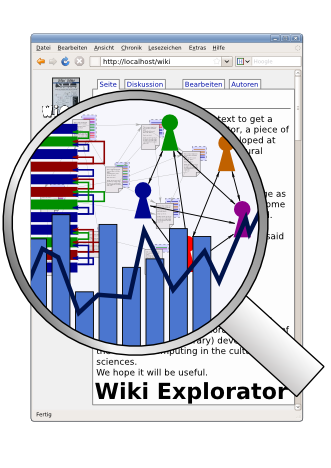
\includegraphics[width=.4\textwidth]{WikiExplorator}\vspace{-1cm}}

\newcounter{fntrdoc}

\begin{document}

\maketitle
\clearpage
\tableofcontents
\clearpage

\section{Introduction}
\label{sec:intro}

In this document I want to give some hints how to use WikiExplorator
in a way that fits your needs. It is a tutorial, not a manual, this
means that all steps given are examples, you will learn one or two
ways to use a certain method or class, but you will not learn about
every possible set of parameters and every method availible. So feel
encuraged to look up the classes and methods used in this tutorial in the
manual\footnote{\url{http://wiki-explorator.rubyforge.org/doc/}}%
\setcounter{fntrdoc}{\thefootnote} and experiment with different
parameter sets.

\section{Installation}
\label{sec:install}

I unpacked the archive to the directory \file{mwparser} and installed
Ruby\footnote{version 1.8.7, version 1.8.6 should also work, if not
  send me a bug report. I testet WikiExplorator on Ruby1.9, but am not
  sure everything works as expected.}, Graphviz, Gnuplot, R, \LaTeX\ and
some Ruby Gems and R packages without problems on (Debian) Linux. For
detailed installation instructions see the \file{INSTALL} file. 

\section{First Steps}
\label{sec:first}

\subsection{Getting Started}
\label{sec:start}

Enter the \file{mwparser} directory and make a copy of
\file{mywikis.rb}. This file will be the personalized startup and
project file, so all customation can be done inside this file. I
recommend to copy this file and save it under another name as
otherwise it would be overwritten when installing new versions.

\begin{typed}
\p{~/mwparser/>} \c{ls} 
html  mediawiki  mediawiki.rb  mywikis.rb  Rakefile.rb  test  util
\p{~/mwparser/>} \c{cp mywikis.rb wio.rb}
\p{~/mwparser/>} \cursor
\end{typed}
I name the new file \file{wio.rb} as our project and its wiki are
named WiO. Now I open \file{wio.rb} with an editor and change it to fit
my environment, looking for the following lines:
\begin{File}
  def Mediawiki.mywiki(pw, options=\{\})
    Wiki.open("wikidb", "localhost", "wikiuser", pw,
              \{:language => 'de', :name => 'MyWiki'\}.merge(options))
  end
\end{File}
Using the class and method documentation\footnotemark[\thefntrdoc] helps
to understand the parameters. The relevant entry is
\rdoc{Mediawiki::Wiki.open}, where some of the parameters are
described and a reference to \rdoc{Mediawiki::DB.new} is given where
the rest of the parameters is documented. To fit everything to my
environment I change the name of the database to \file{wiodb}, give
the database host, the database user and the name and language of the
wiki\footnote{if our tables have some prefix ``\code{xxx}'', we would
  add \cmd{:prefix => 'xxx'} within the braces.}:
\begin{File}
  def Mediawiki.mywiki(pw, options=\{\})
    Wiki.open("wiodb", "wiowiki.kinf.wiai.uni-bamberg.de", "wiouser", pw,
              \{:language => 'de', :name => 'WiO'\}.merge(options))
  end
\end{File}
All of this information can be found by looking into
\file{LocalSettings.php}\footnote{note that \file{localhost} must be
  replaced by the actual hostname if you want to remotely access the
  database. In this case additionally Mysql must allow remote access
  (globally and for this user).}.

So, let's see if everything works:\footnote{the password can also
be found in \file{Localsettings.php}}
\begin{typed}
\p{~/mwparser/>} \c{ruby wio.rb}
Tools for Social Network Analysis
[\dots]

Connecting to your wiki ...
Password: \c{\textit{secret}}

Connecting to your wiki ...
Password: 
connecting to database wiowiki.kinf.wiai.uni-bamberg.de/wiodb
connected.
Table wio_genres in DB not found
Table wio_roles in DB not found
users: 15
revisions: 1362
timeline length: 1352
firsttime: Di Mär 20 18:23:15 UTC 2007
lasttime: Di Jul 28 13:53:09 UTC 2009
Done.
Avg. # of users: 1.8348623853211
# of pages with more than one user: 57/109 (52.29%)

give "report" as command line parameter to create a pdf report of your wiki.

\p{~/mwparser/>} \cursor
\end{typed}
This looks fine. Our wiki has 15 users and 1352 edits, had the first
edit in March 2007 and the last one in July 2009.

\clearpage

\subsection{Interactive usage}
\label{sec:interactive}

So let's see what WikiExplorator can tell about our wiki. We use the
interactive ruby shell \file{irb}:\footnote{instead of \cmd{wio} you
  certainly use whatever you called your project file}
\begin{typed}
\p{~/mwparser/>} \c{irb -r wio}
Tools for Social Network Analysis
\dots
\p{irb(main):001:0>} \cursor
\end{typed}
The parameter ``\code{-r wio}'' means: require the library \code{wio}
which is our project file.

The next step is to open our wiki:
\begin{typed}
\p{irb(main):001:0>} \c{wiki = Mediawiki.mywiki('\textit{secret}')}
connecting to database wiowiki.kinf.wiai.uni-bamberg.de/wiodb
connected.
Table wio_genres in DB not found
Table wio_roles in DB not found
users: 15
revisions: 1362
timeline length: 1352
firsttime: Di Mär 20 18:23:15 UTC 2007
lasttime: Di Jul 28 13:53:09 UTC 2009
Done.
=> #<Mediawiki::Wiki WiO: wiowiki.kinf.wiai.uni-bamberg.de/wiodb, 
271 pages, 1362 revisions, 15 users>
\p{irb(main):002:0>} \cursor
\end{typed}
Now the variable \code{wiki} holds the wiki object (see
\rdoc{Mediawiki::Wiki} in the manual) and we can start to investigate:
\begin{typed}
\p{irb(main):002:0>} \c{wiki.users.length}
=> 15
\p{irb(main):003:0>} \c{wiki.pages.length}
=> 109
\p{irb(main):004:0>} \c{wiki.revisions.length}
=> 1125
\end{typed}
We ask the wiki to give us the users and count their length, we have
15 users, fine. Same for the pages, we have 109 pages. And finally for
the revisions: 1125. But wait! Shouldn't this be 1352? There is
something wrong.

This is caused by the fact that by default only namespace 0 (the main
wiki namespace) is taken into account, so we habe 109 pages and 1125
revisions in namespace 0. We will learn soon how to change this by
using filters (section~\ref{sec:filters}).

\bigskip

For the moment we will see what the wiki can tell us using some
ruby. I cannot provide a full-featured Ruby introduction within this
tutorial but I will try to give some hints.\footnote{use
  \url{http://www.ruby-lang.org/} as a starting point for information
  about Ruby. You may at least need some Ruby knowledge when things
start to get more sophisticated.}

We may also be interested in a single user. Let's fetch the first one
from our wiki's user collection:
\cmd{wiki.users} gives a collection of User objects (see
\rdoc{Mediawiki::User}), and the method \cmd{first} gives the first
entry in this collection:
\begin{typed}
\p{irb(main):005:0>} \c{user = wiki.users.first}
=> #<Mediawiki::User id=5 name="Regina">
\end{typed}
In Ruby every method has a return value and irb indicates the returned
object with ``\code{=>}''. Normally a condensed string representation
of the object is given. 

We could also have asked the wiki for user Regina:
\begin{typed}
\p{irb(main):217:0>} \c{user = wiki.user_by_name('Regina')}
=> #<Mediawiki::User id=5 name="Regina">
\end{typed}
This certainly gives us the same object.

Now we can ask this user a lot of neat things:
\begin{typed}
\p{irb(main):006:0>} \c{user.uid}
=> 5
\p{irb(main):007:0>} \c{user.name}
=> "Regina"
\p{irb(main):008:0>} \c{user.real_name}
=> "Regina Meister"
\p{irb(main):009:0>} \c{user.revisions.length}
=> 105
\p{irb(main):010:0>} \c{user.pages.length}
=> 18
\end{typed}
So Regina has 105 edits on 18 pages. Wouldn't it be nice to have a
list of all users with their pages and edits? We only need to ask each
user for his pages and his revisions, count them and collect this
information:
\begin{typed}
\p{irb(main):011:0>} \c{wiki.users.collect \{ |u|
                     [u.name, u.pages.length, u.revisions.length] \}}
=> [["Regina", 18, 105], ["Sissi", 0, 0], ["system", 1, 1], ["August", 1, 1], 
    ["Tom", 17, 63], ["WikiSysop", 0, 0], ["Fritz", 20, 87], ["Olga", 21, 103],
    ["Klaus", 45, 151], ["Carla", 0, 0], ["Sam", 2, 9], ["Caro", 0, 0], 
    ["Dan", 2, 6], ["Steffen", 71, 594], ["Helga", 2, 5]]
\end{typed}

Some words about the syntax: we ask the wiki object about its users
(call the method \cmd{users} on it), this returns a collection of
users on which we now call the method \cmd{collect} which takes a
block as a parameter. A block is a piece of code given in
braces\footnote{you can also use \cmd{do} \dots\,\cmd{end} instead of
  \cmd{\{} \dots\,\cmd{\}}} taking one or more parameters given in
pipes (\cmd{|u|}). \cmd{collect} calls the block given for every member of
the collection and returns the results of the block in a large array.
\bigskip

Fortunately there is an auxiliary method which pretty prints (pp)
these statistics (the columns are explained in the manual: 
\rdoc{Mediawiki::Wiki.pp\_userstats}):
\begin{typed}
\p{irb(main):013:0>} \c{wiki.pp_userstats}
user         realname                 uid    e    p    e/p   se   fe   ke   ie
===============================================================================
August       August Kaiser              6    1    1   1.00    0    1    0    0
Carla        Carla Schach               8    0    0    nan    0    0    0    0
Caro         Carol Heart                9    0    0    nan    0    0    0    0
Dan          Dan Bosco                 15    6    2   3.00    2    4    0    1
Fritz        Fritz Lost                 7   87   20   4.35   55   27    0    1
Helga        Helga Mayer               10    5    2   2.50    3    1    0    0
Klaus        Klaus Stein                2  151   45   3.36   81   42    0    7
Olga         Olga Kranz                13  103   21   4.90   72   18    0    0
Regina       Regina Meister             5  105   18   5.83   73   31    0    0
Sam          Sam Hawkins               14    9    2   4.50    6    3    0    2
Sissi        Sissi Helfer              11    0    0    nan    0    0    0    0
Steffen      Steffen Blaschke           4  594   71   8.37  458   83    0   27
Tom          Tom Toppler               12   63   17   3.71   43   13    0    0
WikiSysop                               1    0    0    nan    0    0    0    0
system       System User                0    1    1   1.00    0    0    0    0
=> nil
\end{typed}
Hm, and the other way around? How many users on each page?
\begin{typed}
\p{irb(main):031:0>} \c{wiki.pages.collect \{ |p| p.users.length \}}
=> [1, 1, 1, 3, 1, 1, 7, 2, 1, 1, 1, 1, 3, 1, 1, 2, 1, 2, 1, 1, 1, 3, 2, 4, 2, 
    5, 1, 2, 3, 1, 4, 1, 2, 3, 1, 2, 1, 2, 2, 2, 1, 3, 2, 1, 1, 2, 2, 4, 2, 2, 
    2, 4, 1, 5, 1, 2, 2, 1, 1, 1, 2, 2, 1, 1, 1, 2, 1, 3, 2, 2, 1, 2, 1, 2, 1, 
    2, 1, 2, 1, 3, 1, 2, 1, 2, 2, 4, 2, 3, 1, 2, 2, 2, 1, 1, 2, 2, 1, 4, 1, 1, 
    1, 1, 4, 1, 1, 1, 1, 1, 2]
\end{typed}
Not very clear. Perhaps a histogram with the number of pages for each user? 
\begin{typed}
\p{irb(main):037:0>} \c{wiki.pages.collect \{ |p| p.users.length \}.stat_histogram}
=> \{5=>2, 1=>52, 7=>1, 2=>38, 3=>9, 4=>7\}
\end{typed}
That's better, but not good. We try some pseudographics:
\begin{typed}\label{typed:pu}
\p{irb(main):047:0>} \c{pu = wiki.pages.collect \{ |p| p.users.length \}.stat_histogram}
=> \{5=>2, 1=>52, 7=>1, 2=>38, 3=>9, 4=>7\}
\p{irb(main):048:0>} \c{pu.keys.min.upto(pu.keys.max) \{ |k|
                     puts(('%2i: ' % k) + ('#' * pu[k])) \}}
 1: ####################################################
 2: ######################################
 3: #########
 4: #######
 5: ##
 6: 
 7: #
=> 1
\end{typed}
The \cmd{'\%2i:\ '} is a printf expression as known from C.

\clearpage

\begin{figure}
  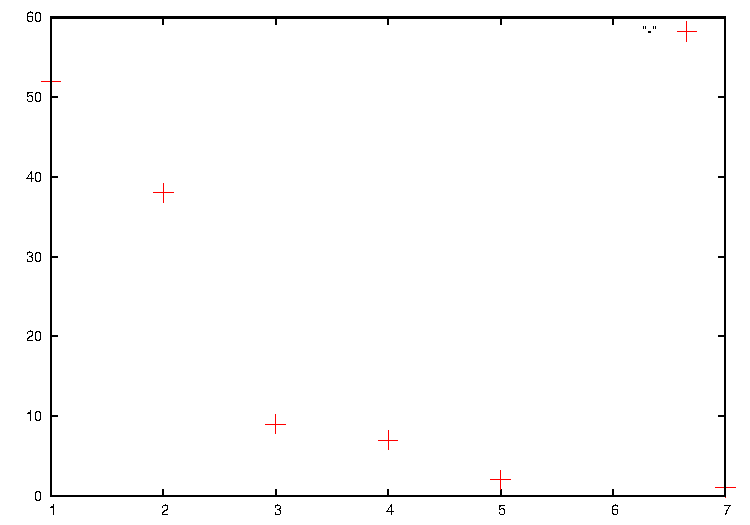
\includegraphics[width=.49\textwidth]{gp_hist_points}\hfill
  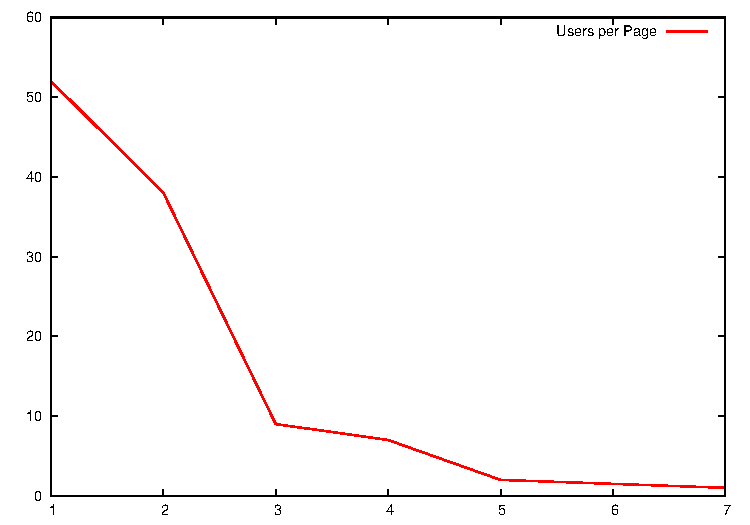
\includegraphics[width=.49\textwidth]{gp_hist_line}\\
  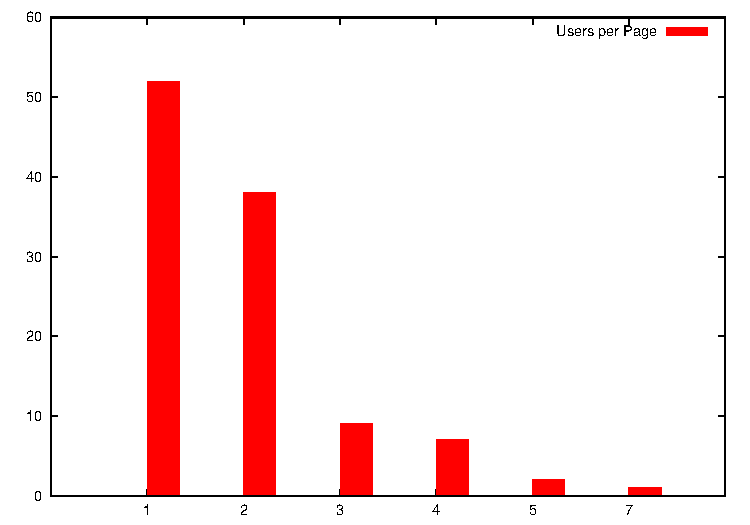
\includegraphics[width=.49\textwidth]{gp_hist_hist0}\hfill
  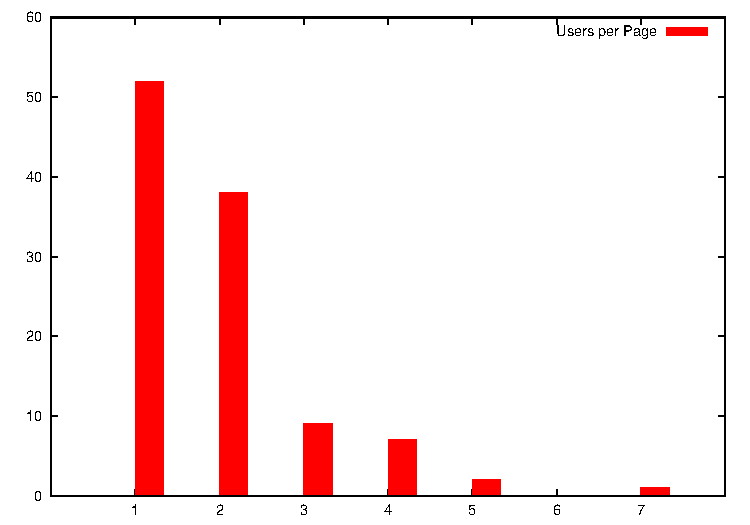
\includegraphics[width=.49\textwidth]{gp_hist_hist}
  \caption{Using Gnuplot for data presentation}
  \label{fig:gp_hist}
\end{figure}

\section{Gnuplot}
\label{sec:gnuplot}

Let's use gnuplot for a graphical representation of this
histogram:\footnote{using \cmd{pu} as defined in session~\ref{typed:pu}}
\begin{typed}
\p{irb(main):051:0>} \c{pu.gp_plot}
=> #<Gnuplot:0xf6733cf4 ... >
\p{irb(main):061:0>} \c{pu.sort.gp_plot(:title => 'Users per Page', :with => 'lines')}
=> #<Gnuplot:0xf66f32a8 ...>
\p{irb(main):070:0>} \c{pu.sort.gp_plot(:title => 'Users per Page',
                     :using => '2:xtic(1)', :with => 'histograms fill solid')}
=> #<Gnuplot:0xf66b60c4 ...>
\end{typed}
First we simply plotted the data using gnuplot
(figure~\ref{fig:gp_hist} top left), then the same using a line and
adding a title (top right). Note that we had to sort the data
before. Try out what happens otherwise. And finally we tried the
histogram (bottom left). It looks fine but has one problem: it would
be nice if we get an empty column with label 6 between 5 and 7. Let's
see how to do this (figure~\ref{fig:gp_hist} bottom right):
\begin{typed}
\p{irb(main):072:0>} \c{(pu.keys.min..pu.keys.max).collect \{ |k| [k, pu[k]]
                      \}.gp_plot(:title => 'Users per Page',
                      :using => '2:xtic(1)', :with => 'histograms fill solid')}
=> #<Gnuplot:0xf66807d0 ...>
\end{typed}
\begin{figure}
  \parbox[b]{.5\textwidth}{%
  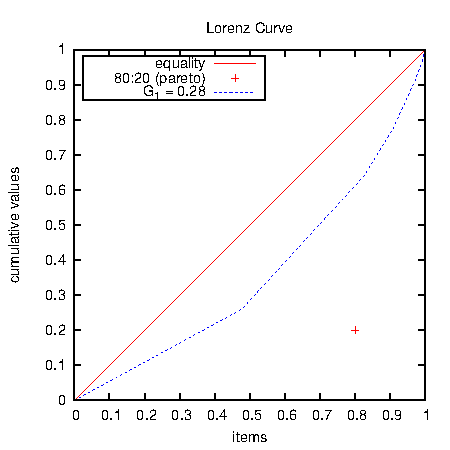
\includegraphics[width=\linewidth]{gp_lorenz}
  \caption{Lorenz curve for users per page}
  \label{fig:gp_lorenz}}\hfill
  \parbox[b]{.485\textwidth}{%
  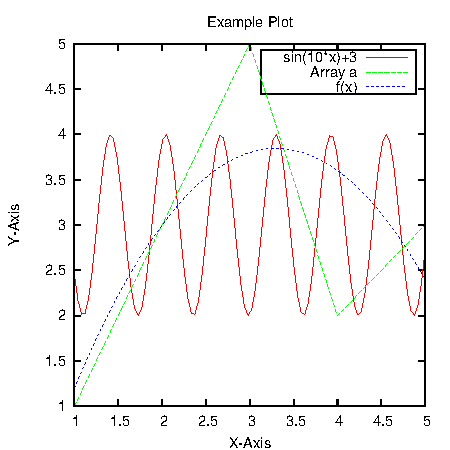
\includegraphics[width=\linewidth]{gp_example}\vspace{1mm}
  \caption{Extended gnuplot example}
  \label{fig:gp_example}}
\end{figure}
On the other hand, the data (users per page) is as if predestined to
be presented as a Lorenz
curve\footnote{\url{http://en.wikipedia.org/wiki/Lorenz_curve}}, so
let's see what we get (figure~\ref{fig:gp_lorenz}):
\begin{typed}
\p{irb(main):107:0>} \c{wiki.pages.collect \{ |p| p.users.length \}.gp_plot_lorenz}
=> #<Gnuplot:0xf64c3258 ...
 ... lines and lines of output ...
 ... >
\end{typed}
Nice picture. But irb disturbed me with printing so many lines of
output for the gnuplot object. We can fix this by adding another
command with less output (we just use nil):
\begin{typed}
\p{irb(main):107:0>} \c{wiki.pages.collect \{ |p| p.users.length \}.gp_plot_lorenz; nil}
=> nil
\end{typed}
Fine. But gnuplot is more. See
\url{http://gnuplot.sourceforge.net/demo_4.2/} for examples about what
gnuplot can do. And certainly all of this is accessible from
WikiExplorator, including function fitting etc. (see also the examples
in \rdoc{Gnuplot.new}, \rdoc{Gnuplot.fit}). I give you a small example
for extended gnuplot usage at figure~\ref{fig:gp_example} using an
array \cmd{a} and the function \cmd{$\sin(10x)+3$}:
\begin{typed}
\p{irb(main):111:0>} \c{a = [[1,1], [2,3], [3,5], [4,2], [5,3]]}
=> [[1, 1], [2, 3], [3, 5], [4, 2], [5, 3]]
\p{irb(main):127:0>} \c{Gnuplot.new do |gp|}
\p{irb(main):128:1*} \c{  gp.add('sin(10*x)+3')}
\p{irb(main):129:1>} \c{  gp.add(a, :with => 'lines', :title => 'Array a')}
\p{irb(main):130:1>} \c{  gp.fit(:function => 'f(x) = a*x**2 + b*x + c', :via => 'a,b,c')}
\p{irb(main):131:1>} \c{  gp.title = 'Example Plot'}
\p{irb(main):132:1>} \c{  gp.set('key','box')}
\p{irb(main):133:1>} \c{  gp.set('xlabel', 'X-Axis', true)}
\p{irb(main):134:1>} \c{  gp.set('ylabel', 'Y-Axis', true)}
\p{irb(main):135:1>} \c{  gp.plot}
\p{irb(main):136:1>} \c{end}
...
=> #<Gnuplot:0xf7a5e3c4 ... >
\end{typed}
So one thing is left: we want the graphics to be saved, either as
bitmap or as vector graphics. So let's plot our example array \cmd{a}
to file\footnote{\label{fnt:pspdf}you may need to use \cmd{:pspdf} instead of
  \cmd{:pdf} if your gnuplot has no native PDF support}:
\begin{typed}
\p{irb(main):184:0>} \c{a.gp_plot(:with => 'lines', :png => 'example.png')}
=> #<Gnuplot:0xf6753400 ...>
\p{irb(main):185:0>} \c{a.gp_plot(:with => 'lines', :svg => 'example.svg')}
=> #<Gnuplot:0xf674c920 ...>
\p{irb(main):186:0>} \c{a.gp_plot(:with => 'lines', :pdf => 'example.pdf')}
=> #<Gnuplot:0xf6745c74 ...>
\end{typed}

\clearpage

\begin{figure}
  \parbox[b]{.5\textwidth}{%
    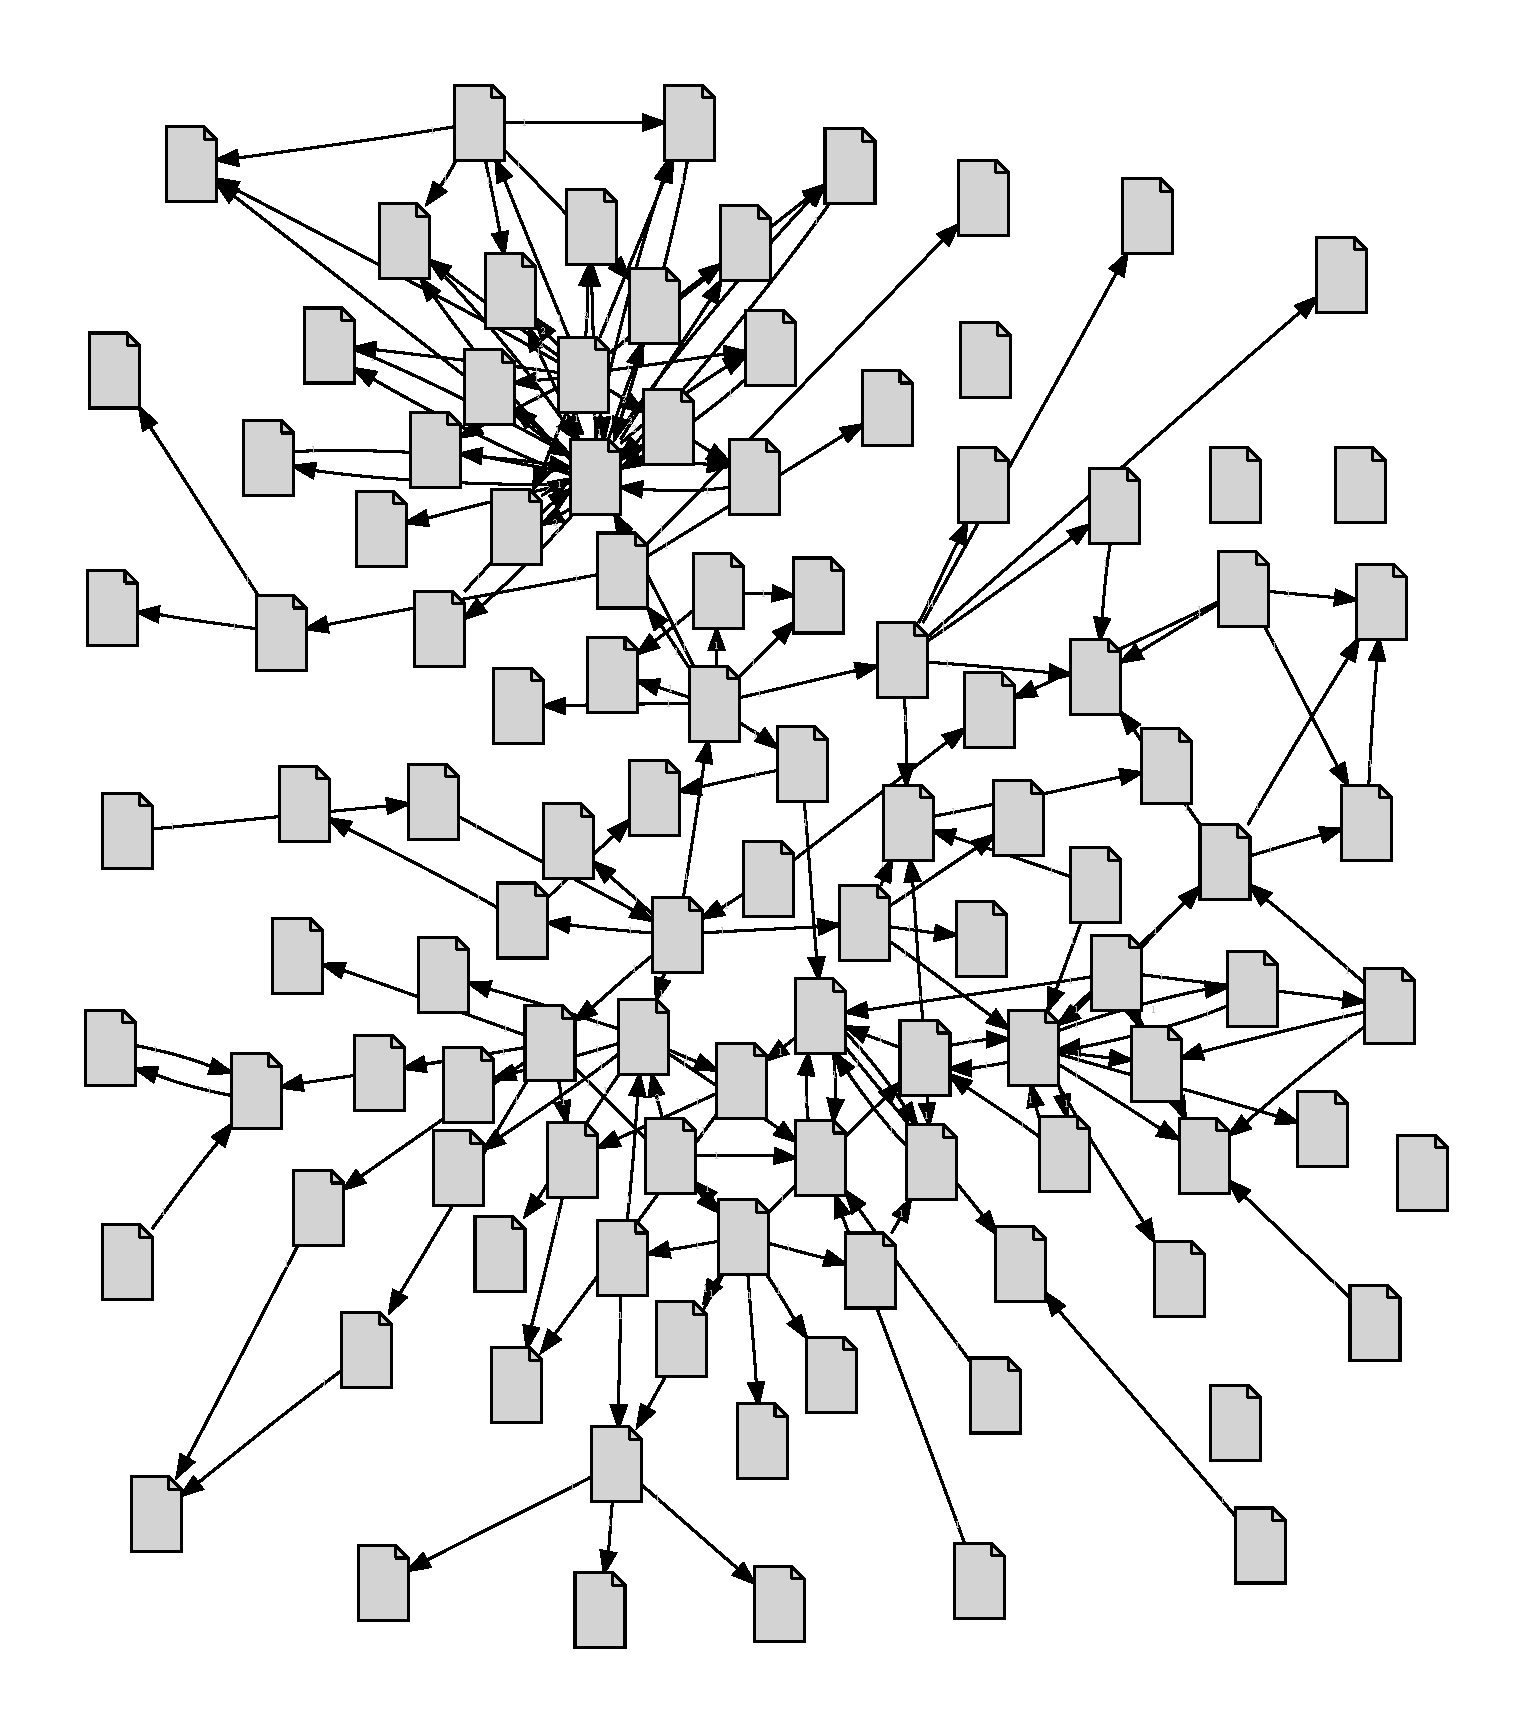
\includegraphics[width=\linewidth]{gv_pagegraph}
    \caption{hyperlink network}
    \label{fig:hyperlink}
  }%
  \parbox[b]{.5\textwidth}{%
    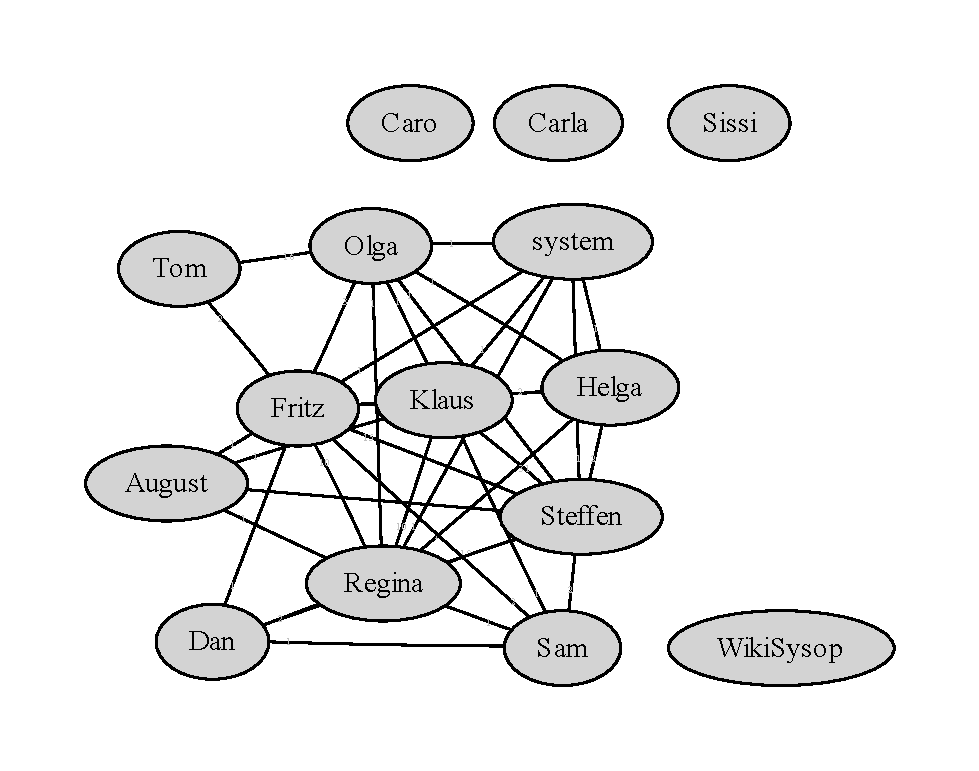
\includegraphics[width=\linewidth]{gv_coauthorgraph-full}\vspace{1cm}
    \caption{coauthorship network}
    \label{fig:coauthor}
  }
\end{figure}

\section{Network Graphs}
\label{sec:network}

Many aspects of a wiki can be represented as networks. The most
obvious networks are the page hyperlink graph
(figure~\ref{fig:hyperlink}) where the nodes represent the wiki pages
and the (directed) edges give the links between the pages, and the
coauthorship network (figure~\ref{fig:coauthor}) where the nodes
represent the wiki authors and two authors are connected with a link
if they edited the same page.\footnote{more precisely: two authors are
  connected by an edge if there exists at least one page both did at
  least edit once.}

As we will see soon a lot of varieties of these as well as different
graphs are available.

\subsection{First Steps}
\label{sec:dotgraphintro}

We start with asking the wiki for the coauthorshipgraph:
\begin{typed}
\p{irb(main):030:0>} \c{cgraph = wiki.coauthorgraph}
=> #<DotGraph:0xf779a2c8 ...>
\end{typed}
This gives us a \cmd{DotGraph} object representing the network. 
This DotGraph object can now be used to compute various network
measures and to visualize the graph in different ways.
Most of the methods work on directed and undirected graphs, some also
respect edge weights.

We start with
some statistics about the degree distribution, sorted by user name
(\rdoc{DotGraph.pp\_degrees}):
\begin{typed}
\p{irb(main):049:0>} \c{cgraph.pp_degrees(:sortby => :node, :up => true)}
Node                          :  deg
August                        :    4
Carla                         :    0
Caro                          :    0
Dan                           :    4
Fritz                         :   10
Helga                         :    6
Klaus                         :    8
Olga                          :    7
Regina                        :    9
Sam                           :    5
Sissi                         :    0
Steffen                       :    9
Tom                           :    2
WikiSysop                     :    0
system                        :    6
=> nil
\end{typed}
So Fritz is connected to most of the others, directly followed by
Regina and Steffen. On a second thought, we are not interested on
nodes not connected to others, so we remove them, and then we print
our list again, now with user real names and sorted by degree:
\begin{typed}\label{typed:remove_lonely_nodes}
\p{irb(main):065:0>} \c{cgraph.remove_lonely_nodes; nil}\footnotemark
=> nil
\p{irb(main):066:0>} \c{cgraph.pp_degrees(:sortby => :degree) \{ |u| u.real_name \}}
Node                          :  deg
Fritz Lost                    :   10
Steffen Blaschke              :    9
Regina Meister                :    9
Klaus Stein                   :    8
Olga Kranz                    :    7
Helga Mayer                   :    6
System User                   :    6
Sam Hawkins                   :    5
August Kaiser                 :    4
Dan Bosco                     :    4
Tom Toppler                   :    2
=> nil
\end{typed}
That's better. Now the ranking is obvious.%
\footnotetext{You remember: the \cmd{nil} is only given to suppress
  the (rather lengthy) return output}
We used the \code{pp\_degrees} method in the example to get pretty
output (\code{pp} stands for ``pretty print''). For further processing
we could have used \code{degrees} which gives the raw data. Some but
not all methods have \code{pp\_} counterparts for convenience. So when
I use a \code{pp\_} method in the following examples have a look at
the pure method.

\subsection{R}
\label{sec:Rintro}

If \file{R} and \file{rsruby} are installed and working (and the
required \file{R} libraries are installed) we can access all of the
network measures \file{R} (or rather the \file{R} library \file{sna})
provides using ruby. The method documentation states which
\code{DotGraph} methods are based on \file{R}. So we can
e.\,g. compute betweenness, closeness and others (for full
\file{R} access see section~\ref{sec:Rfull}):%
\begin{typed}
\p{irb(main):093:0>} \c{cgraph.pp_betweenness(:sortby => :value)}
Node                          :          betweenness
============================================================
Fritz                         :         8.8333333333
Steffen                       :         3.3333333333
Regina                        :         3.3333333333
Olga                          :         2.5000000000
Klaus                         :         1.7500000000
Sam                           :         0.2500000000
Helga                         :         0.0000000000
Dan                           :         0.0000000000
August                        :         0.0000000000
Tom                           :         0.0000000000
system                        :         0.0000000000
=> nil
\p{irb(main):094:0>} \c{cgraph.pp_closeness(:sortby => :value)}
Node                          :            closeness
============================================================
Fritz                         :         1.0000000000
Steffen                       :         0.9090909091
Regina                        :         0.9090909091
Klaus                         :         0.8333333333
Olga                          :         0.7692307692
Helga                         :         0.7142857143
system                        :         0.7142857143
Sam                           :         0.6666666667
August                        :         0.6250000000
Dan                           :         0.6250000000
Tom                           :         0.5555555556
=> nil
\end{typed}

\subsection{Graph Visualization}
\label{sec:gvis}

\begin{figure}
\parbox[b]{0.7\textwidth}{
  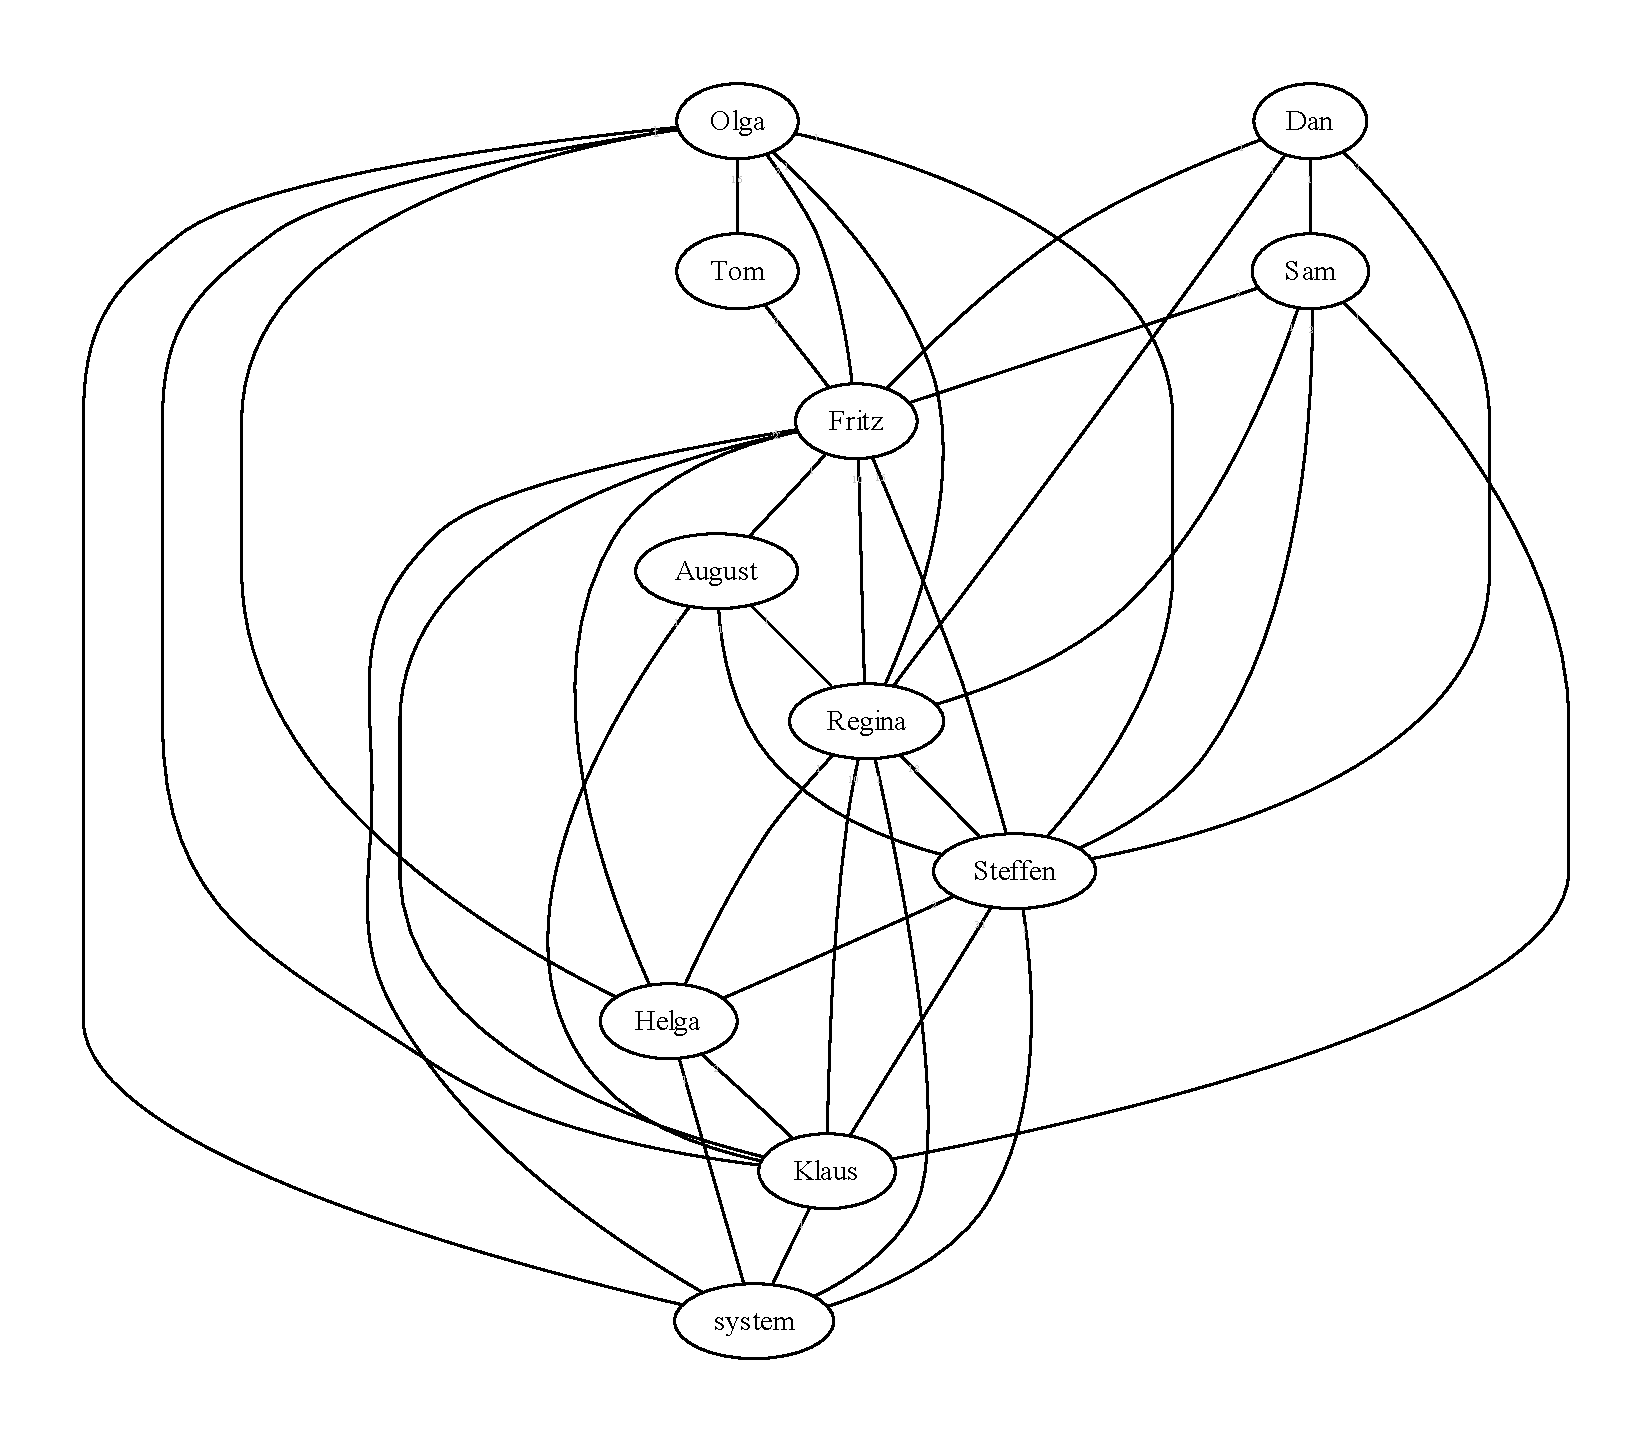
\includegraphics[width=\linewidth]{gv_ca-dot}\vspace{-7mm}
  \caption{\code{dot} layout}
  \label{fig:gv-cadot}}%
\parbox[b]{0.3\textwidth}{\centering
  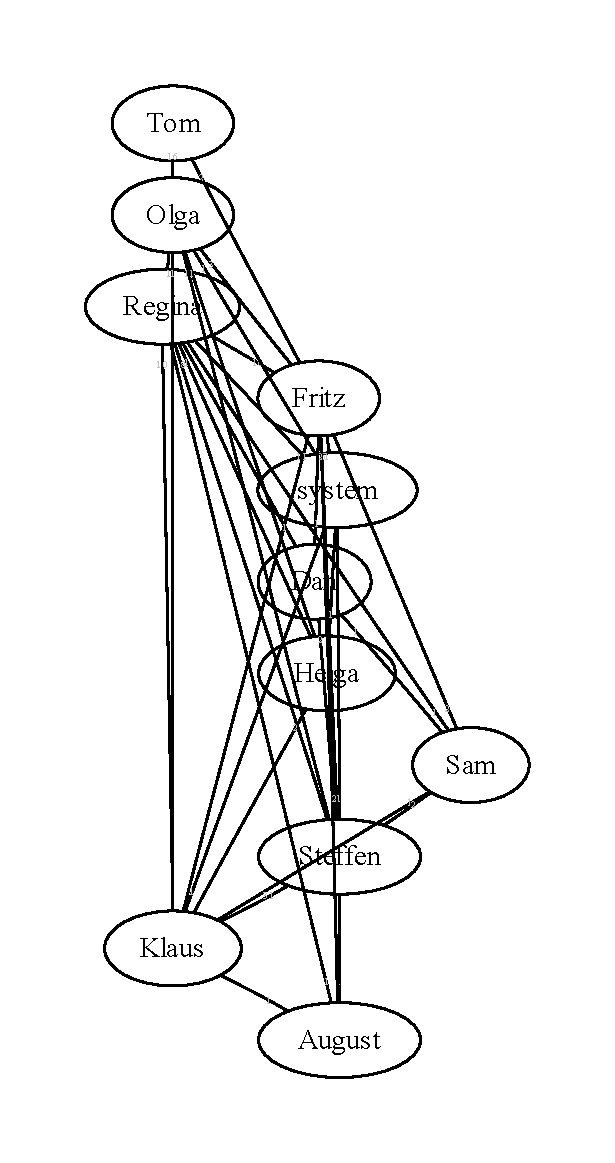
\includegraphics[width=\linewidth]{gv_ca-fdp}
  \caption{\code{fdp} layout}
  \label{fig:gv-cafdp}}\\
\parbox[b]{0.7\textwidth}{\centering
  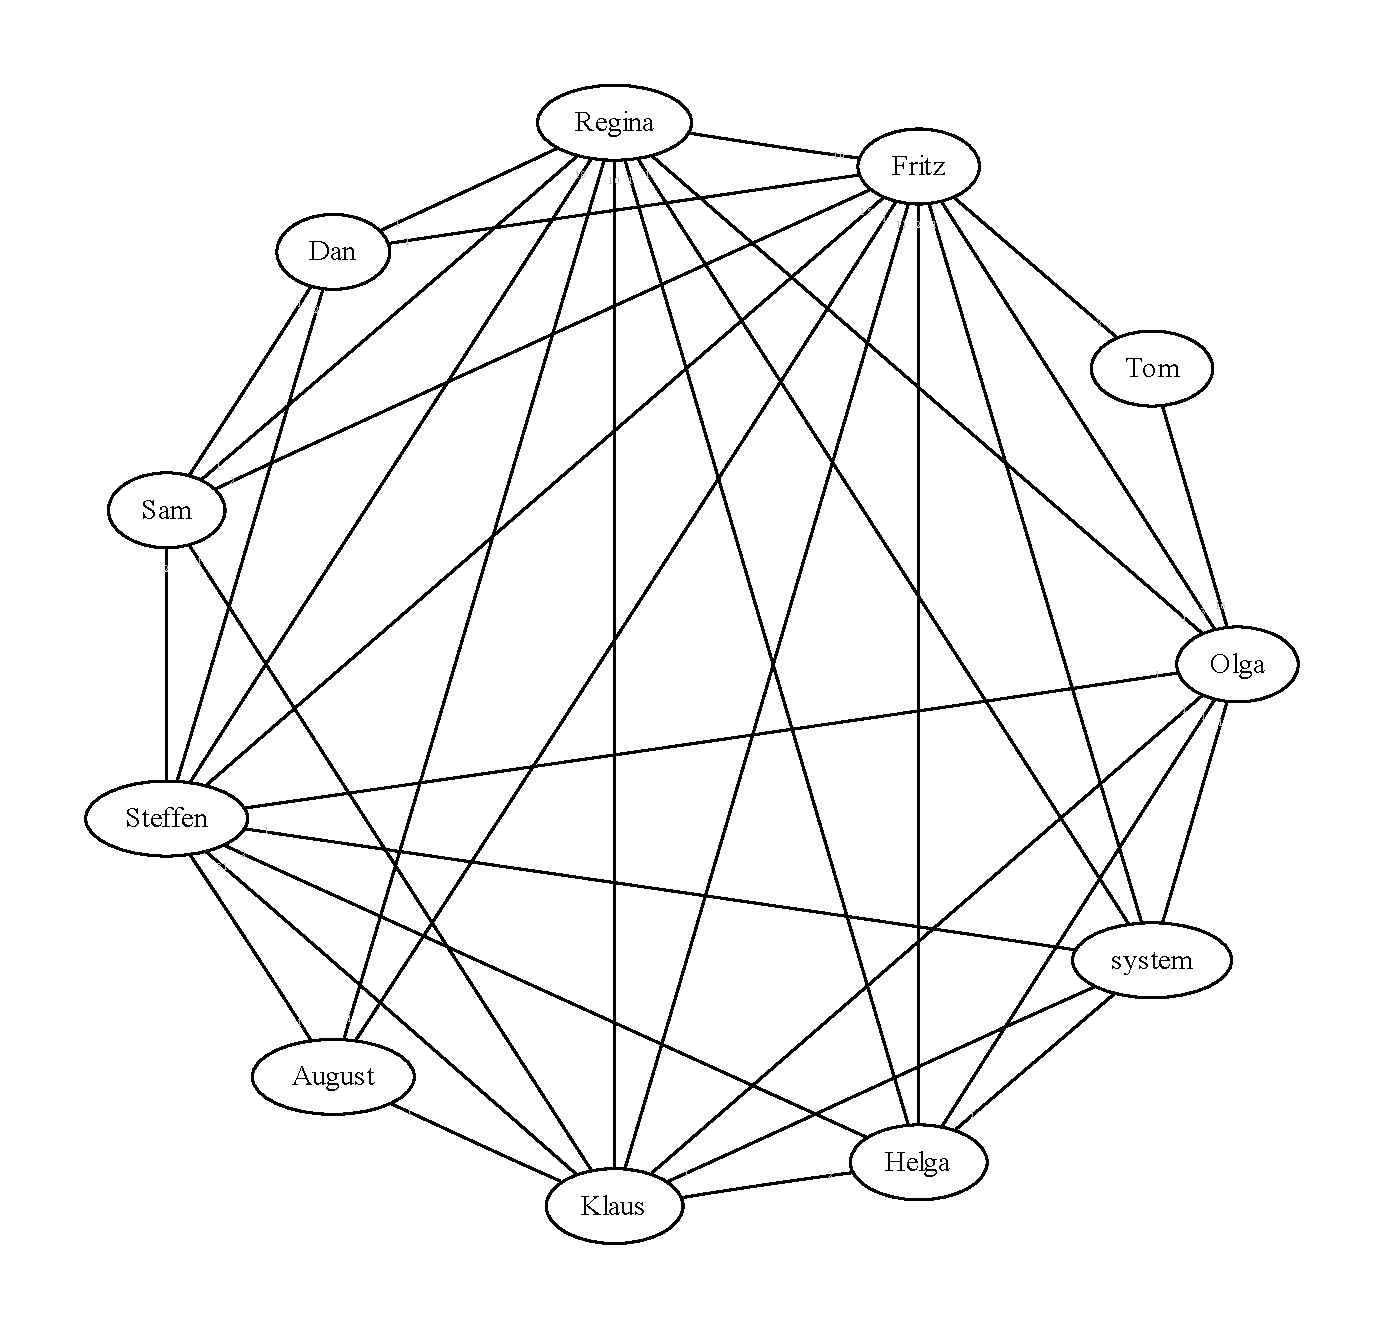
\includegraphics[width=\linewidth]{gv_ca-circo}\vspace{-7mm}
  \caption{\code{circo} layout}
  \label{fig:gv-cacirco}}%
\parbox[b]{0.3\textwidth}{\centering
  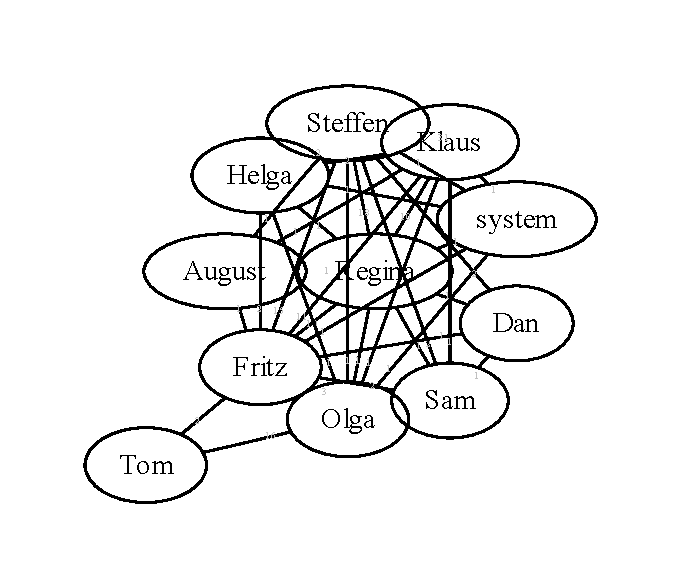
\includegraphics[width=\linewidth]{gv_ca-twopi}\vspace{-7mm}
  \caption{\code{twopi} layout}
  \label{fig:gv-catwopi}
  \vspace{8mm}

  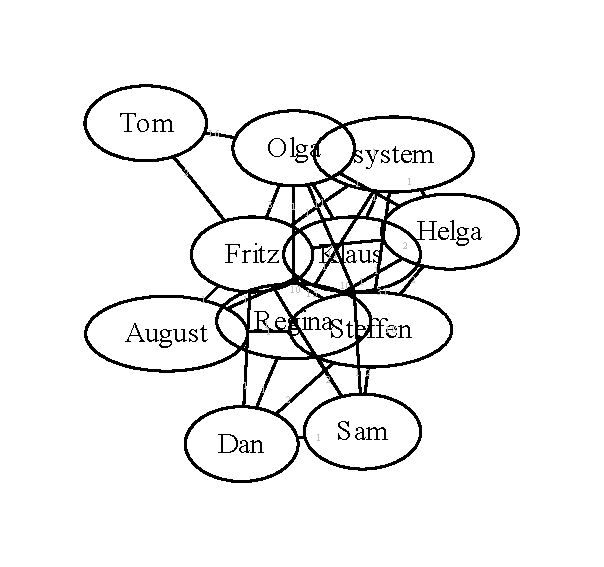
\includegraphics[width=\linewidth]{gv_ca-neato}\vspace{-7mm}
  \caption{\code{neato} layout}
  \label{fig:gv-caneato}}
\end{figure}

Network statistics are fine but we would rather be interested to see
some nice graphics. WikiExplorator can create graph visualizations in
different ways and with different layout algorithms using either
\file{graphviz} or \file{R}.

\subsubsection{Graphviz}
\label{sec:graphviz}

\file{graphviz} can be used in two ways: if \file{ruby-graphviz}
(module \file{gv}) is present it is used, otherwise it is silently
substituted by calls to the \file{graphviz} executables.\footnote{the
  main drawback here is that it is slow.} We start by using the
different graphviz layout engines\footnote{see the \file{graphviz} manpage and
\url{http://www.graphviz.org/} for details} and create some PDFs:\footnote{(you may need to use \cmd{:pspdf} instead, see
  footnote~\ref{fnt:pspdf}, Sec.\,\ref{sec:gnuplot}), others
  (SVG, PNG, \dots) are available.}
\begin{typed}
\p{irb(main):107:0>} \c{cgraph.to_graphviz('gv_ca-dot.pdf','dot', :pdf)}
=> true
\p{irb(main):108:0>} \c{cgraph.to_graphviz('gv_ca-fdp.pdf','fdp', :pdf)}
=> true
\p{irb(main):109:0>} \c{cgraph.to_graphviz('gv_ca-circo.pdf','circo', :pdf)}
=> true
\p{irb(main):110:0>} \c{cgraph.to_graphviz('gv_ca-twopi.pdf','twopi', :pdf)}
=> true
\p{irb(main):111:0>} \c{cgraph.to_graphviz('gv_ca-neato.pdf','neato', :pdf)}
=> true
\end{typed}
This gives the graphs in figures~\ref{fig:gv-cadot}
to~\ref{fig:gv-caneato}.\footnote{These graphs as well as the
  statistics before do not include the unconnected nodes visible in
  figure~\ref{fig:coauthor} as we removed them in session~\ref{typed:remove_lonely_nodes}.}  These graphs obviously need some
finetuning. For the \code{twopi} (fig.\,\ref{fig:gv-catwopi}) and
\code{neato} (fig.\,\ref{fig:gv-caneato}) layout the nodes overlap,
and for \code{fdp}, \code{twopi} and \code{neato}
(fig.\,\ref{fig:gv-cafdp}--\ref{fig:gv-caneato}) the edges go across
the nodes. By passing additional parameters to graphviz we can solve
this (see the graphviz documentation for available options):

\begin{figure}
\parbox[b]{0.5\textwidth}{\centering
  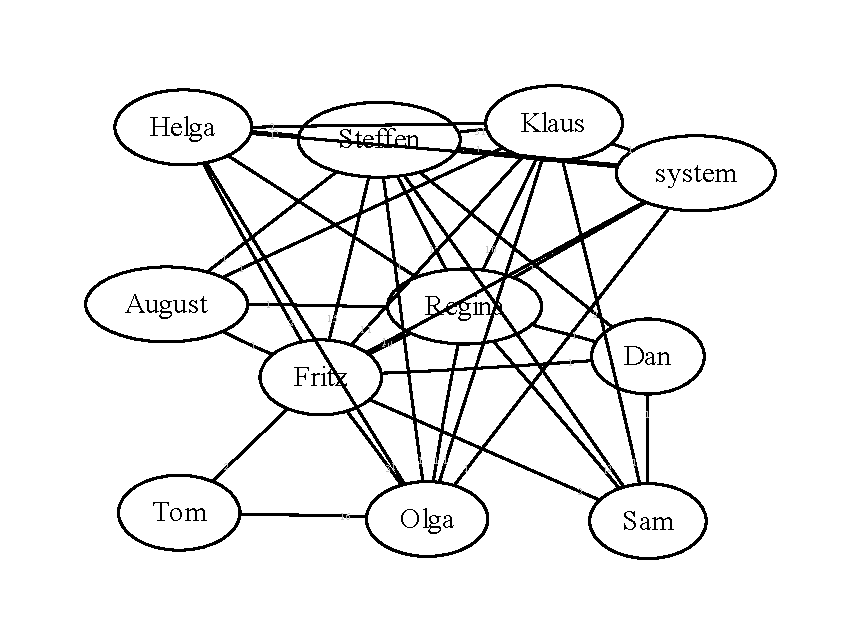
\includegraphics[width=\linewidth]{gv_ca-twopi-ol}\vspace{-1cm}
  \caption{\code{twopi} without overlap}
  \label{fig:gv-catwopi2}}%
\parbox[b]{0.5\textwidth}{\centering
  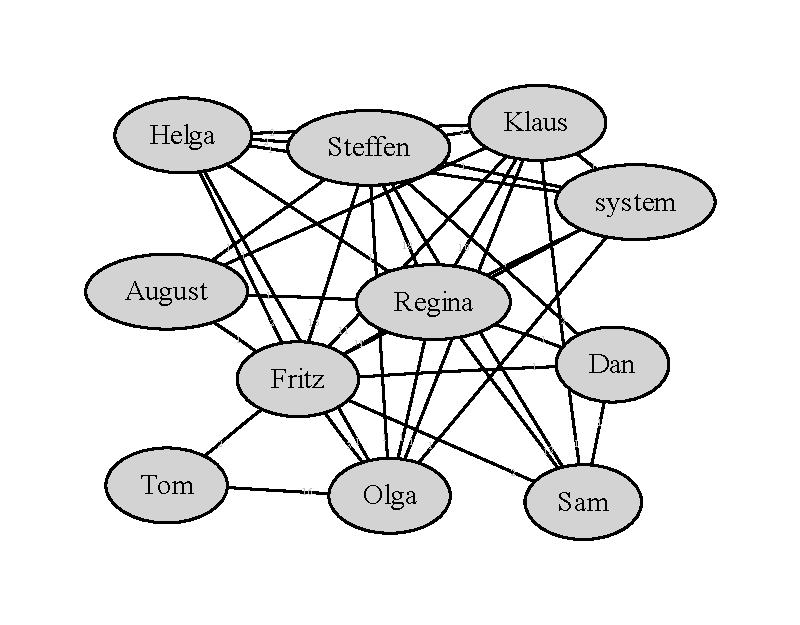
\includegraphics[width=\linewidth]{gv_ca-twopi-olf}\vspace{-1cm}
  \caption{\code{twopi}: nodes in front of edges}
  \label{fig:gv-catwopi3}}
\end{figure}

\begin{typed}
\p{irb(main):112:0>} \c{cgraph.to_graphviz('gv_ca-twopi-ol.pdf', 'twopi', :pdf, 
                                    'overlap=false')}
=> true
\p{irb(main):113:0>} \c{cgraph.to_graphviz('gv_ca-twopi-olf.pdf', 'twopi', :pdf, 
                                    'overlap=false', 'outputorder=edgesfirst', 
                                    'node [style=filled]')}
=> true
\end{typed}
The first call\footnote{\cmd{'overlap=false'} tells graphviz to shift
  the nodes apart from each other} gives figure~\ref{fig:gv-catwopi2},
the second\footnote{\cmd{'outputorder=edgesfirst'} tells graphviz to
  first draw the edges, so the nodes are printed over the edges. This
  only has an effect if the nodes are solid, so we add \cmd{'node
    [style=filled]'}} figure~\ref{fig:gv-catwopi3}. Try the same for
\code{fdp} and \code{neato}!
\begin{figure}
\parbox[b]{0.5\textwidth}{\centering
  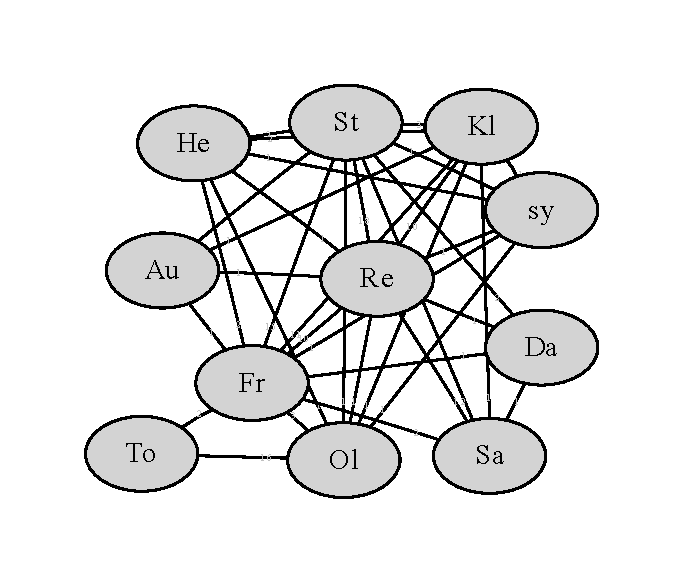
\includegraphics[width=\linewidth]{gv_ca-twopi-olf-short}
  \caption{\code{twopi}: short labels}
  \label{fig:gv-catwopi4}}%
\parbox[b]{0.5\textwidth}{\centering
  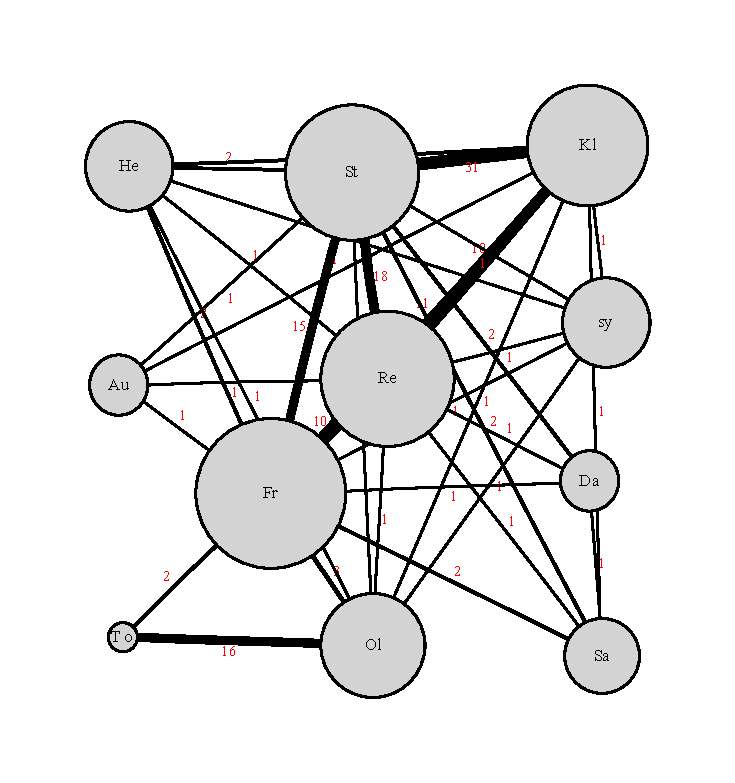
\includegraphics[width=\linewidth]{gv_ca-twopi-degwidth}\vspace{-1cm}
  \caption{\code{twopi}: weighted sizes}
  \label{fig:gv-catwopi5}}
\end{figure}
Currently the nodes have different size as the names (node labels) are
of different length. Perhaps we should abbreviate all labels to two
characters: 
\begin{typed}
\p{irb(main):115:0>} \c{cgraph.nodeblock \{ |node| node.name[0..1] \}}
=> #<Proc:0xf5ecf748@(irb):115>
\p{irb(main):116:0>} \c{cgraph.to_graphviz('gv_ca-twopi-olf-short.pdf', 'twopi', :pdf, 
                                    'overlap=false', 'outputorder=edgesfirst', 
                                    'node [style=filled]')}
=> true  
\end{typed}
In the first line we set the \code{nodeblock} of this graph. The
nodeblock is called for each node to create its label and should
either return a string (used as label) or an array (used as node
parameters). See \rdoc{DotGraph.nodeblock} for details.

I used this to create the hyperlink graph
(figure~\ref{fig:hyperlink}):
\begin{typed}
\p{irb(main):018:0>} \c{wiki.pagegraph \{''\}.to_graphviz('pagegraph.pdf', 'neato', :pdf, 
                     'outputorder=edgesfirst', 'overlap=false', 
                     'node [shape=note, style=filled, width=.34]')}
=> #<IO:0xf765e454>
\end{typed}
Here the nodeblock is given on creation and returns an empty string
for any node. By adding some width and shape directives I got these
nice paper icons as node shapes to represent our wiki pages.

And for completeness, here is figure~\ref{fig:coauthor} (we create a
new coauthorgraph from the wiki, so here the unconnected nodes are not
removed and therefore displayed in the graph):
\begin{typed}
\p{irb(main):028:0>} \c{wiki.coauthorgraph.to_graphviz('gv_coauthorgraph-full.pdf',
                     'neato', :pdf, "outputorder=edgesfirst", "overlap=false", 
                     "node [style=filled]")}
=> #<IO:0xf7a7554c>
\end{typed}

Finally, we want to compute node sizes dependent on node degrees and
edge width dependent on link weights\footnote{\cmd{coauthorgraph}
  weights edges between authors with the number of pages they are
  coauthors on.}:
\begin{typed}
\p{irb(main):161:0>} \c{cgraph.nodeblock \{ |node| 
                                    size = (cgraph.n_degree(node)/10.0).to_s; 
                                    ["label=#\{node.name[0..1]\}", 
                                     'width=' + size, 'height=' + size] \}}
=> #<Proc:0xf5c80dd4@(irb):161>
\p{irb(main):173:0>} \c{cgraph.to_graphviz('gv_ca-twopi-degwidth.pdf', 'twopi', :pdf, 
                     'overlap=false', 'outputorder=edgesfirst',
                     'node [fontsize=8, style=filled, fixedsize]') \{ |weight| 
                        ["penwidth=#\{weight**0.5\}", "label=#\{weight\}", 
                         'fontsize=7', 'fontcolor=red' ] \}}
Warning: node 'u6', graph 'G' size too small for label
Warning: node 'u12', graph 'G' size too small for label
Warning: node 'u15', graph 'G' size too small for label
=> #<IO:0xf5bb9950>
\end{typed}
We first set the nodeblock. We use the degree of the node to compute
the \cmd{size}: we ask \cmd{cgraph} for the degree of the node and
divide it by 10.0.\footnote{the divisor has to be a Float, otherwise
  ruby would use Integer division} The method \cmd{to\_s} converts the
result to string. Now we asseble an array with three entries: the node
label set to the first two characters of the user name, the node width
and the node height, both set to \cmd{size}.\footnote{You may notice
  usage of single (\cmd{'}) and double (\cmd{"}) quotes. This is
  similar to shells like sh or bash: strings in double quotes
  (\cmd{"}) are subject to substitution, in our example this means
  that the result of the ruby code given in \cmd{\#\{\dots\}} is
  inserted in the string.}  And finally we ask \cmd{cgraph} to create
the graph. You may notice that we appended an additional block to this
call. This block is called for each edge with the edge weight as
parameter, similar to nodeblock.

Graphviz allows much more than the few examples shown
here,\footnote{see the gallery at
  \url{http://www.graphviz.org/Gallery.php}}, if you find expressive
and impressive visualizations feel free to send me examples (source
code and graphics). The parameters are described at
\url{http://www.graphviz.org/doc/info/attrs.html}, the graphviz
homepage provides elaborate user manuals for all layout
algorithms. Use \cmd{to\_dotfile} to see the outcome of the parameters:
\begin{typed}
\p{irb(main):218:0>} \c{cgraph.to_dotfile('cgraph.dot', 'outputorder=edgesfirst',
                     'overlap=false', 'node [style=filled]')  \{ |weight| 
                            ["penwidth=#\{weight**0.5\}", "label=#\{weight\}"] \}}
=> #<File:~/mwparser/cgraph.dot (closed)>
\end{typed}
The resulting file \file{cgraph.dot} can be opened with any text editor.

%WikiExplorator may write graphs in \code{dot} format you can also
%use these to directly experiment with the graphviz toolbox.

Lets close with one final example. We use (nearly) the same parameters
as before and just change the layout engine (figure~\ref{fig:gv-catcirco}):
\begin{figure}[t]
  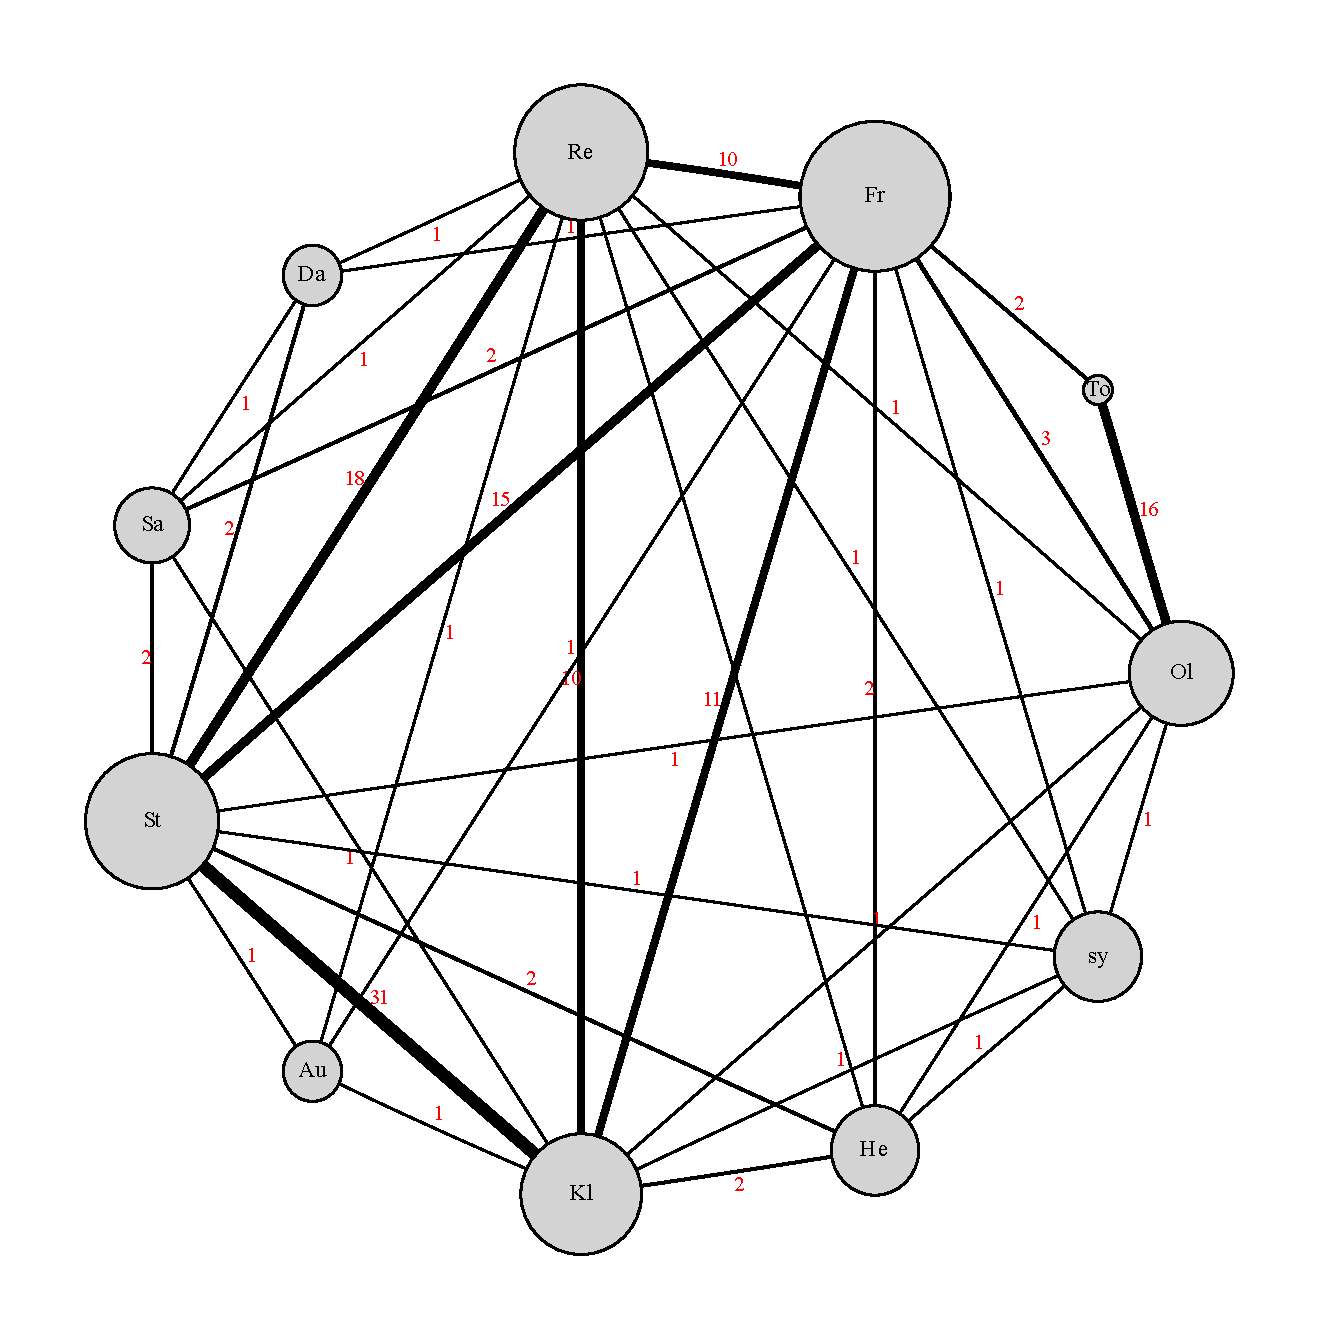
\includegraphics[width=\linewidth]{gv_ca-circo-degwidth}\vspace{-1cm}
  \caption{\code{circo}: weighted sizes}
  \label{fig:gv-catcirco}
\end{figure}
\begin{typed}
\p{irb(main):180:0>} \c{cgraph.to_graphviz('gv_ca-circo-degwidth.pdf', 'circo', :pdf, 
                     'overlap=false', 'outputorder=edgesfirst', 
                     'node [fontsize=11, style=filled, fixedsize]')  \{ |weight|
                        ["penwidth=#\{weight**0.5\}", "label=#\{weight\}", 
                         'fontsize=10', 'fontcolor=red' ] \}}
Warning: node 'u6', graph 'G' size too small for label
Warning: node 'u12', graph 'G' size too small for label
Warning: node 'u15', graph 'G' size too small for label
=> #<IO:0xf5b7fc00>
\end{typed}

\subsubsection{R}
\label{sec:vizR}

Graphviz allows for rather pretty and sophisticated graph prints, but
has the drawback not to display graphs on screen (which was rather
convenient with gnuplot). Thankfully we can use \code{R} for this
(figure~\ref{fig:r_coauthor}):
\begin{typed}
\p{irb(main):182:0>} \c{dev = cgraph.r_plot}
=> 2
\p{irb(main):183:0>} \c{cgraph.r_plot_close(dev)}
=> {"null device"=>1}
\end{typed}
\begin{figure}
  \parbox[b]{0.37\textwidth}{%
    \centering
    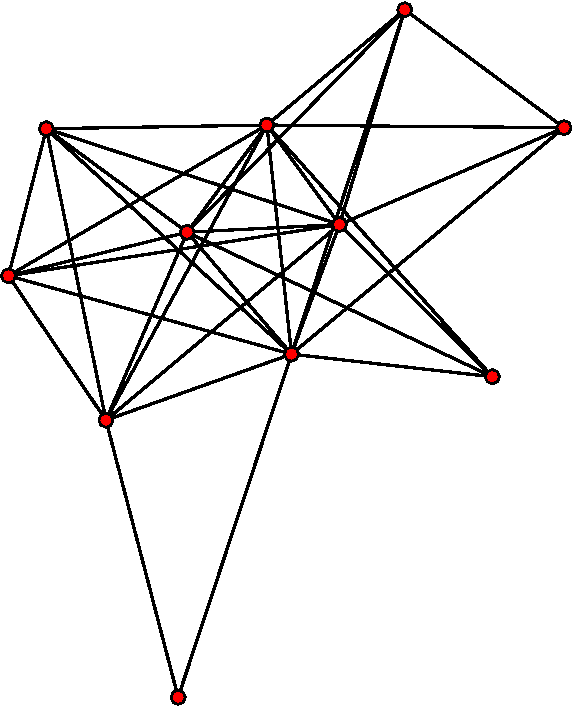
\includegraphics[width=\linewidth]{r_coauthor}
    \caption{Plotting using \code{R}}
    \label{fig:r_coauthor}
  }
  \parbox[b]{0.63\textwidth}{%
    \centering
    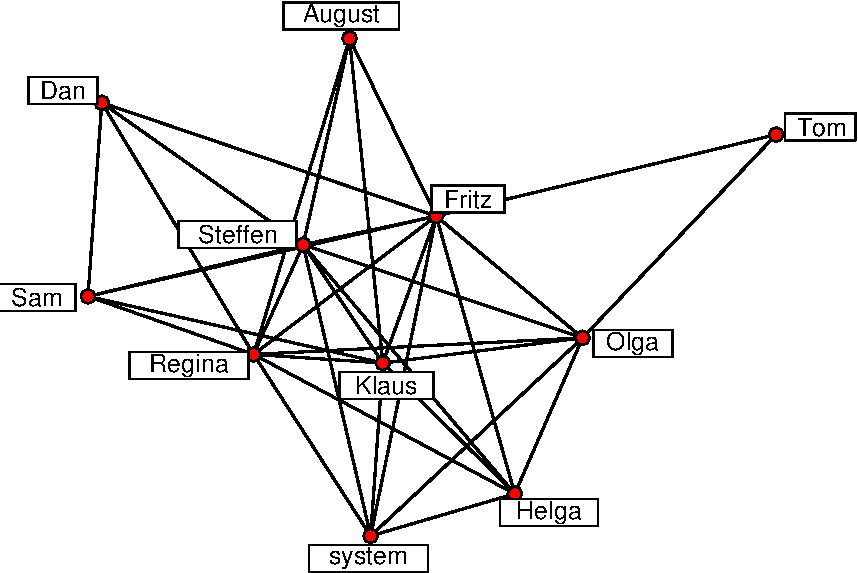
\includegraphics[width=\linewidth]{r_coauthor2}
    \caption{Plotting with labels using \code{R}}
    \label{fig:r_coauthor2}
  }
\end{figure}
As you can see \cmd{cgraph.r\_plot} returns a number which indicates
the \code{R} plot device and which can be used to close the graph
window. On some OS you may just close the window using its close
button, on others this does not work, there you have to use
\cmd{r\_plot\_close}.

Unfortunately changing attributes can get somehow cumbersome using
\code{R} syntax, well, at least for me, if you know \code{R} from
heart things may be different for you
(figure~\ref{fig:r_coauthor2}):\footnote{this example uses
  \cmd{DotGraph.r\_plot\_close} which works as well and ist independent
  of a certain graph object.}
\begin{typed}
\p{irb(main):190:0>} \c{cgraph.r_plot(:displaylabels => TRUE,
                     :label => lambda \{ |nw,r| 
                        r.get_vertex_attribute(nw, "attr")\}) \{ |u| u.name \}}
=> 2
\p{irb(main):191:0>} \c{DotGraph.r_plot_close(2)}
=> {"null device"=>1}
\end{typed}
So I use \cmd{r\_plot} for a fast interactive graph overview and stay
with graphviz for prints.

\section{Using Filters}
\label{sec:filters}

Enough of playing with graphs and networks, back to the wiki.

As stated before the wiki is not seen raw but through a view which is
customized by a filter. Filters are the way to see cutouts of a wiki,
including or excluding certain users, namespaces, and to go back in
time, to see how the wiki looked like years ago or what happened
within a certain timespan.

\subsection{First steps}
\label{sec:filters-first}

When asking the wiki for the number of pages by default I only get
pages from the main namespace (0). But we certainly can change this:
\begin{typed}
\p{irb(main):199:0>} \c{wiki.pages.length}
=> 109
\p{irb(main):200:0>} \c{wiki.filter.include_all_namespaces}
=> #<Set: {0, 6, 1, 2, 8, 14, 3, 4, 10}>
\p{irb(main):201:0>} \c{wiki.pages.length}
=> 271
\end{typed}
We first ask the wiki for its pages. After that \cmd{wiki.filter}
gives us the active filter of the wiki on which we call the method
\cmd{include\_all\_namespaces}. As we can see from the return value
this automagically collects all namespaces found in the wiki. And
finally we ask the wiki again for its pages, and suddenly their number
raises from 109 to 271.
\bigskip

We have two users in our wiki who are not part of our normal staff:
``system'' and ``WikiSysop''.\footnote{While the ``WikiSysop'' is an
  ordinary wiki user with special rights, the ``system'' user is
  special. It does not show up in the user database and you cannot
  login as ``system'' user, but it is owner of all revisions done
  internally by Mediawiki (e.\,g. as result of mass uploads etc.).  }
Perhaps we should exclude them from our statistics:
\begin{typed}
\p{irb(main):230:0>} \c{f = wiki.filter}
=> #<Mediawiki::Filter:0xf7669e6c ...>
\p{irb(main):231:0>} \c{wiki.revisions.length}
=> 1362
\p{irb(main):232:0>} \c{wiki.user_by_name('system').revisions.length}
=> 2
\p{irb(main):233:0>} \c{wiki.user_by_name('WikiSysop').revisions.length}
=> 1
\p{irb(main):234:0>} \c{f.deny_user('system', 'WikiSysop')}
=> ["system", "WikiSysop"]
\p{irb(main):235:0>} \c{wiki.revisions.length}
=> 1359
\end{typed}
We ask the wiki for its filter and save it in \cmd{f}. The wiki
currently has 1362 revisions, the ``system'' user has two revisions
and ``WikiSysop'' has one. Now we tell the filter to exclude these two
users and the wiki shows us 1359 ($=1362-2-1$) revisions, so this
looks fine.

\bigskip

How does this work? Well, when we ask the wiki for its users, we get a
UsersView of the wiki which uses the given filter:
\begin{typed}
\p{irb(main):240:0>} \c{users = wiki.users}
=> #<Mediawiki::UsersView:0xf5d4dba4 ...>
\p{irb(main):241:0>} \c{users.length}
=> 13
\p{irb(main):242:0>} \c{f.undeny_user('WikiSysop')}
=> ["WikiSysop"]
\p{irb(main):243:0>} \c{users.length}
=> 14
\end{typed}
What we see here is that changing the filter affects the corresponding
view.


\subsection{Multiple filters}
\label{sec:filter-dup}

In the last section we changed the current filter of the wiki to get
different views. This does not work if we want to deal with different
views in parallel: we need more than one filter. So let's copy our
current filter and see what we can do with it:
\begin{typed}
\p{irb(main):244:0>} \c{f2 = f.clone}
=> #<Mediawiki::Filter:0xf5d43618 ...>
\p{irb(main):245:0>} \c{f2.namespace = 0}
=> 0
\p{irb(main):246:0>} \c{wiki.revisions(f2).length}
=> 1124
\p{irb(main):247:0>} \c{wiki.revisions.length}
=> 1360
\end{typed}
We use \cmd{clone} to get a real copy of the filter \cmd{f} and save
it in \cmd{f2},\footnote{cloning is important, otherwise both
  varfiables would point to the \emph{same} object!} after that we
restrict the namespace of \cmd{f2} to 0 and then we use \cmd{f2} for
the \cmd{revisions} view. Any method of Wiki returning a view as well
as many of the other methods\footnote{i.\,e. graph generation and
  statistics methods} take a filter as optional
parameter.\footnote{send a bug report if I missed a method.}

A cloned filter inherits the attributes of the original
one. Alternatively we can create a clean filter for our wiki:
\begin{typed}
\p{irb(main):249:0>} \c{f3 = Mediawiki::Filter.new(wiki)}
=> #<Mediawiki::Filter:0xf5cf2628 ...>
\end{typed}
So \cmd{f3} has all attributes set to start values (namespace 0, no
excluded users, \dots).

See \rdoc{Mediawiki::Filter} to learn about filter attributes.

\subsection{Back and forth in time}
\label{sec:filter-time}

One nice feature of a wiki is the page history. We can reconstruct how
the wiki looked like months or years ago, and we do this using
filters.

So let's see how the wiki looked like a year ago:
\begin{typed}
\p{irb(main):260:0>} \c{f3.revision_timespan}
=> Di Mär 20 18:23:15 UTC 2007..Di Jul 28 13:53:09 UTC 2009
\p{irb(main):261:0>} \c{f3.endtime = '2008-8-1'}
=> "2008-8-1"
\p{irb(main):262:0>} \c{f3.revision_timespan}
=> Di Mär 20 18:23:15 UTC 2007..Fr Aug 01 00:00:00 +0200 2008
\p{irb(main):266:0>} \c{wiki.pages(f3).length}
=> 84
\p{irb(main):268:0>} \c{wiki.pages(f2).length}
=> 109
\end{typed}
Initially \cmd{f3} includes the whole timespan from March 20, 2007 to
July 28, 2009. We set the endtime to August 1, 2008 and ask again for
the timespan, fine, worked like expected.

Now we ask the wiki for the pages within this timespam (84) and
compare it to the number of pages until now (109). So obviously we got
25 ($=109-84$) new pages added in the last year.

Ok, how many revisions within the last four weeks?
\begin{typed}
\p{irb(main):270:0>} \c{f3.full_timespan}
=> Di Mär 20 18:23:15 UTC 2007..Di Jul 28 13:53:09 UTC 2009
\p{irb(main):271:0>} \c{f3.starttime = f3.endtime - 60*60*24*7*4}
=> Di Jun 30 13:53:09 UTC 2009
\p{irb(main):272:0>} \c{f3.revision_timespan}
=> Di Jun 30 13:53:09 UTC 2009..Di Jul 28 13:53:09 UTC 2009
\p{irb(main):273:0>} \c{wiki.revisions(f3).length}
=> 10
\end{typed}
We first set \cmd{f3} to full timespan, set the new starttime by
subtracting four weeks in seconds from the endtime, controlled that it
worked and asked for the number of revisions. Not much traffic in our
example wiki the last four weeks.

Wouldn't it be nice to have this for the whole timeline? That's easy
as the wiki helps us generating a custom timeraster:
\begin{typed}\label{typed:revtr}
\p{irb(main):270:0>} \c{f3.full_timespan}
=> Di Mär 20 18:23:15 UTC 2007..Di Jul 28 13:53:09 UTC 2009
\p{irb(main):275:0>} \c{tr = wiki.timeraster(:step => :week, :zero => :week)}
=> [So Mär 18 00:00:00 +0100 2007, So Mär 25 00:00:00 +0100 2007, ...,
                                     ..., So Aug 02 01:00:00 +0200 2009]
\p{irb(main):279:0>} \c{ r1 = tr.collect \{ |t| f3.endtime = t; 
                                        [t, wiki.revisions(f3).length] \}}
=> [[So Mär 18 00:00:00 +0100 2007, 0], [So Mär 25 00:00:00 +0100 2007, 18], ...,
                                     ..., [So Aug 02 01:00:00 +0200 2009, 1125]]
\p{irb(main):284:0>} \c{r1.gp_plot(:with => 'lines'); nil}
=> nil
\end{typed}
First we reset \cmd{f3} to full timespan (again). Then we ask the wiki
to generate a weekly timeraster and use this timeraster to compile an
array of arrays with the endtime as first and the number of revisions
up to this time as second entry. And finally we use gnuplot to plot
the revision growth in time (figure~\ref{fig:gp_revtr}).

\begin{figure}
  \parbox[b]{.5\textwidth}{%
  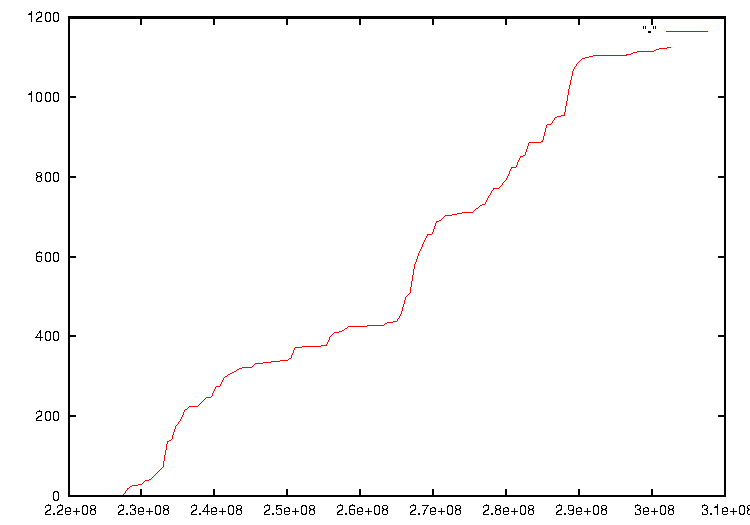
\includegraphics[width=\linewidth]{gp_revtr}
  \caption{weekly revisions (cumulative)}
  \label{fig:gp_revtr}}
  \parbox[b]{.5\textwidth}{%
  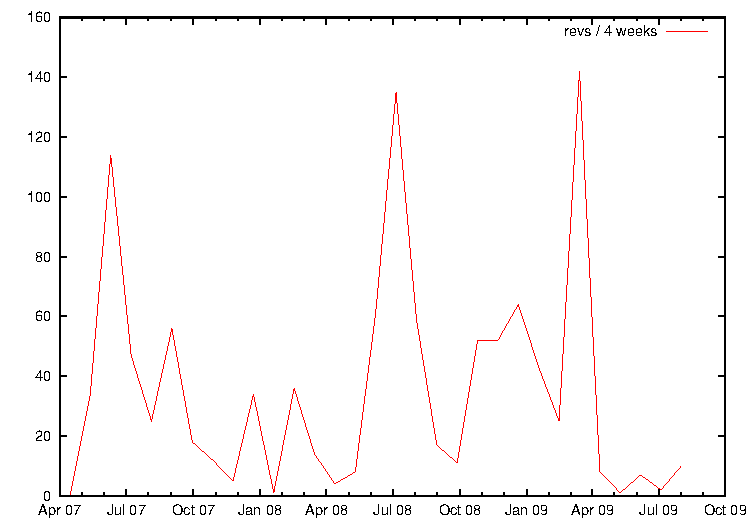
\includegraphics[width=\linewidth]{gp_revtr2}
  \caption{monthly revisions}
  \label{fig:gp_revtr2}}
\end{figure}

In the last example we only changed endtime, so the number of
revisions grew. Now we want to see how the number of new revisions
changes in time. The following example could be written slightly more
simple when using the \file{enumerator} module available in ruby 1.8.7
and later (see \rdoc{Mediawiki::Wiki.timeraster} for an example using
enumerator). We use a time raster of four weeks:
\begin{typed}
\p{irb(main):339:0>} \c{tr = wiki.timeraster(:step => 60*60*24*7*4, :zero => :week)}
=> [So Mär 18 00:00:00 +0100 2007, So Apr 15 01:00:00 +0200 2007, ...]
\p{irb(main):340:0>} \c{start = tr.shift}
=> So Mär 18 00:00:00 +0100 2007
\p{irb(main):341:0>} \c{r2 = tr.collect \{ |t| f3.revision_timespan = (start..t); 
                                       start = t; 
                                       [t, wiki.revisions(f3).length] \}}
=> [[So Apr 15 01:00:00 +0200 2007, 0], ... ]
\p{irb(main):381:0>} \c{Gnuplot.new do |gp|}
\p{irb(main):382:1*} \c{  gp.set('xdata', 'time')}
\p{irb(main):383:1>} \c{  gp.set('timefmt', '%Y-%m-%d', true)}
\p{irb(main):384:1>} \c{  gp.set('format x', '%b %y', true)}
\p{irb(main):385:1>} \c{  gp.add(r2, :with => 'lines', :title => 'revs / 4 weeks',
                              :timefmt => '%Y-%m-%d')}
\p{irb(main):386:1>} \c{  gp.plot}
\p{irb(main):387:1>} \c{end}
=> #<Gnuplot:0xf5d8a61c ...>
\end{typed}
As you can see I put some efforts in gnuplot to get nice formatted output.
So I hope you got an idea about what filters can do for you, even if
sometimes the direct way is faster (this results in a graph very close
to session~\ref{typed:revtr} (figure~\ref{fig:gp_revtr}):
\begin{typed}
\p{irb(main):416:0>} \c{c = 0; wiki.revisions.sort_by \{ |r| r.timestamp \}.collect \{ |r| 
                             [r.timestamp, c += 1] \}.gp_plot(:with => 'lines')}
\end{typed}
Here we directly use the revision timespans to generate the graph.

\clearpage

\section{ToDo}
\label{sec:todo}

\begin{itemize}
\item user aliasing
\item Full R access (manual, \file{r.rb})
\item further graph generation methods
\item sonia
\item loading and dumping (marshal, yaml), obliterate
\item more sophisticated examples
\item scripting
\item customized reports (html, \LaTeX)
\item conclusion/summary/overview/architecture
\end{itemize}

\end{document}
